\documentclass{article}
\usepackage{amsmath}
\usepackage{amsfonts}
\usepackage{amssymb}
\usepackage{graphicx}
\usepackage{booktabs}
\usepackage{hyperref}
\usepackage{xcolor}
\hypersetup{
    colorlinks,
    linkcolor={red!50!black},
    citecolor={blue!50!black},
    urlcolor={blue!80!black}
}
\usepackage[a4paper, total={6in, 8in}]{geometry}
\usepackage{libertine}
\usepackage{multirow}

\usepackage{tikz}
\usetikzlibrary{trees}

\newcommand{\n}{n}

\newcommand{\nregions}{\n^{\text{reg}}}
\newcommand{\nconnections}{\n^{\text{conn}}}

\newcommand{\ncore}{\n^\text{core}}
\newcommand{\ncopy}{\n^\text{copy}}

\newcommand{\state}{x}
\newcommand{\stateCore}{x}
\newcommand{\stateCopy}{z}

\newcommand{\pf}{g^{\text{pf}}}
\newcommand{\busspecs}{g^{\text{bus}}}

\newcommand{\norm}[1]{\left\lVert#1\right\rVert}

%opening
\title{Morenet documentation}
\author{Tillmann Mühlpfordt}

\begin{document}

\maketitle

\begin{abstract}
This documents sketches the idea to solve the distributed power flow problem as a distributed nonlinear least-squares problem.
\end{abstract}

\section{Problem formulation}
The mathematical formulation for the decentralized power flow problem reads
\begin{subequations}
    \label{eq:dist-power-flow-problem}
    \begin{align}
        \pf_i( \stateCore_i, \stateCopy_i ) &= 0, \\
        \busspecs_i ( \stateCore_i ) &= 0, \\
        \sum_{i = 1}^{\nregions} A_i \begin{bmatrix}
            \stateCore_i \\
            \stateCopy_i
        \end{bmatrix}
        &= 0,
    \end{align}
\end{subequations}
where the consensus matrices $A_i \in \mathbb{R}^{4 \nconnections \times (4 \ncore_i + 2 \ncopy_i)}$ enforce equality of the voltage angle and the voltage magnitude at the copy buses and their respective original buses.
Mathematically speaking, Problem~\ref{eq:dist-power-flow-problem} is a system of nonlinear equations; there are as many equations as there are unknowns.
In principle, Problem~\ref{eq:dist-power-flow-problem} can be solved by Newton's method.
However, we would like to explore alternatives to Newton's method, such as distributed optimization.

\section{Problem solution}
Currently, we solve Problem~\ref{eq:dist-power-flow-problem} as a \emph{distributed feasibility problem}, namely
\begin{subequations}
    \label{eq:dist-feasibility-problem}
    \begin{align}
        \underset{\stateCore_i, \stateCopy_i \, \forall i \in  \{1, \dots, \nregions\}}{\operatorname{min}} \: 0 \quad \operatorname{s.t.}\\
        \pf_i( \stateCore_i, \stateCopy_i ) &= 0, \\
        \busspecs_i ( \stateCore_i ) &= 0, \\
        \sum_{i = 1}^{\nregions} A_i \begin{bmatrix}
            \stateCore_i \\
            \stateCopy_i
        \end{bmatrix}
        &= 0.
    \end{align}
\end{subequations}
From our experience so far, we can say that Aladin is a viable method, but ADMM is not.
Solving a distributed feasibility problem, however, is not the only way.
We can also think of solving Problem~\ref{eq:dist-power-flow-problem} as a \emph{distributed least-squares problem} of the form
\begin{subequations}
    \label{eq:dist-least-squares-problem}
    \begin{align}
        \underset{\stateCore_i, \stateCopy_i \, \forall i \in  \{1, \dots, \nregions\}}{\operatorname{min}} \sum_{i = 1}^{\nregions}  \: \norm{\begin{bmatrix}
            \pf_i( \stateCore_i, \stateCopy_i ) \\
            \busspecs_i ( \stateCore_i )
        \end{bmatrix}}^2 \quad \operatorname{s.t.} ~ \sum_{i = 1}^{\nregions} A_i \begin{bmatrix}
            \stateCore_i \\
            \stateCopy_i
        \end{bmatrix}
        = 0.
    \end{align}
\end{subequations}
Clearly, the solution to Problem~\ref{eq:dist-feasibility-problem} is the solution to Problem~\ref{eq:dist-least-squares-problem} (why?).
Hence, we can think of solving the least-squares Problem~\ref{eq:dist-least-squares-problem} as a necessary condition.

\subsection{Next steps}

The goal is to explore how to solve the distributed power flow problem via a distributed least-sqaures Problem~\ref{eq:dist-least-squares-problem}.
To do so, there are a couple of immediate next steps
\begin{itemize}
    \item Familiarize with nonlinear least-squares (Gauss-Newton, Levenberg-Marquardt, etc)
    \item Solve a prototypical distributed power flow problem.
    \item Use the Jacobian matrix that is given analytically as a return value from \href{https://iai-vcs.iai.kit.edu/advancedcontrol/code/morenet/morenet/-/blob/master/03_parser/generate_distributed_problem.m}{\texttt{generate$\_$distributed$\_$problem}}.
    \item Work out how the Aladin algorithm simplifies in the absence of both equality and inequality constraints. (Note that inequality constraints in the form of lower/upper bounds might still be necessary, i.e. $\underline{x} \leq x \leq \overline{x}$)
    \item Exploit the problem structure as much as possible. As a general rule, the bigger the problem, the more it pays off to exploit sparsity etc.
\end{itemize}

Another thing to explore is to interface Ipopt directly from Matlab.
This is somewhat painful to \href{https://projects.coin-or.org/Ipopt/wiki/MatlabInterface}{set up} but might be worth the speed up anyhow.

\autoref{fig:Algorithm-tree} shows all possible \emph{paths} that are worth taking.
Insights thus far are

\begin{itemize}
    \item The path ``feasibility problem~\eqref{eq:dist-feasibility-problem} $>$ ADMM'' is a dead end; this is a valuable insight in itself.
    \item The path ``feasibility problem~\eqref{eq:dist-feasibility-problem} $>$ Aladin'' works with
    \begin{itemize}
        \item Casadi \& Ipopt for small problems ($< 300$ buses total) in a reasonable time; Casadi is the main bottleneck, Ipopt is not.
        \item fmincon for medium-sized problems ($< 1000$ buses total); fmincon becomes simply too slow.
    \end{itemize}
    \item The path ``least-squares problem~\eqref{eq:dist-least-squares-problem} $>$ ADMM'' has not been explored yet.
    \item The path ``least-squares problem~\eqref{eq:dist-least-squares-problem} $>$ Aladin'' is being investigated, and promising.
\end{itemize}

% \begin{table}
%     \centering
%     \caption{Our experience so far with solving Problem~\ref{eq:dist-power-flow-problem}. A ``---'' indicates further investigations are required.\label{tab:knowledge-base}}
%     \begin{tabular}{llllp{4cm}}
%         \toprule
%         Method & Solver & Number of iterations & Wall clock time & Remark\\
%         \midrule
%         ADMM & Casadi \& Ipopt & many & not acceptable\\
%         \midrule
%         \multirow{5}{*}{Aladin} & Casadi \& Ipopt & few & acceptable & does not scale well to larger problems ($N \approx 100$)\\
%          & fmincon \& Jacobian & few & acceptable & tends to become slow for larger problems ($N \approx 300$)\\
%          & Ipopt \& Jacobian & --- & --- & ---\\
%          \midrule
%         Least squares & --- & --- & --- & ---\\
%         \bottomrule
%     \end{tabular}
% \end{table}

\tikzstyle{every node}=[draw=black,thick,anchor=west]
\begin{figure}
    \centering
    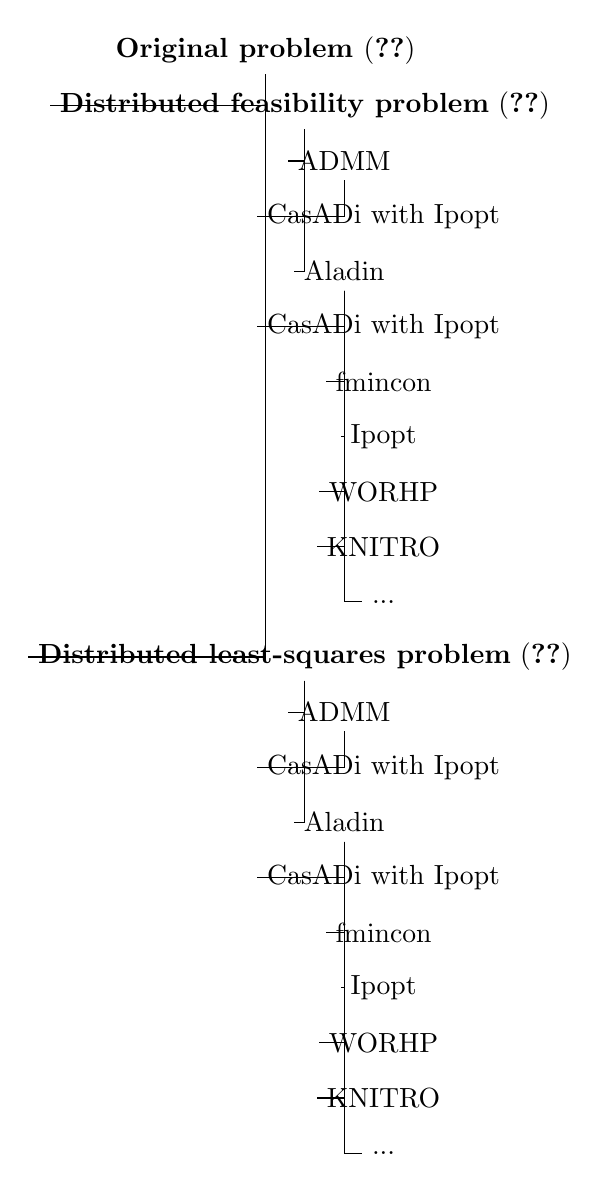
\begin{tikzpicture}[%
      grow via three points={one child at (0.5,-0.7) and
      two children at (0.5,-0.7) and (0.5,-1.4)},
      edge from parent path={(\tikzparentnode.south) |- (\tikzchildnode.west)}]
      \node {\textbf{Original problem~\eqref{eq:dist-power-flow-problem}}}
        child { node {\textbf{Distributed feasibility problem}~\eqref{eq:dist-feasibility-problem}}
            child { node{ADMM}
                child { node{CasADi with Ipopt}}
            }
            child [missing] {}
            child { node{Aladin}
                child { node{CasADi with Ipopt}}
                child { node{fmincon}}
                child { node{Ipopt}}
                child { node{WORHP}}
                child { node{KNITRO}}
                child { node{...}}
            }
        }
        child [missing] {}
        child [missing] {}
        child [missing] {}
        child [missing] {}
        child [missing] {}
        child [missing] {}
        child [missing] {}
        child [missing] {}
        child [missing] {}	
        child { node {\textbf{Distributed least-squares problem}~\eqref{eq:dist-least-squares-problem}}
            child { node{ADMM}
                child { node{CasADi with Ipopt}}
            }
            child [missing] {}
            child { node{Aladin}
                child { node{CasADi with Ipopt}}
                child { node{fmincon}}
                child { node{Ipopt}}
                child { node{WORHP}}
                child { node{KNITRO}}
                child { node{...}}
            }
        };
    \end{tikzpicture}
    \caption{Variants of tackling the distributed power flow problem~\eqref{eq:dist-power-flow-problem}.\label{fig:Algorithm-tree}}
\end{figure}
\end{document}
